\documentclass[11pt]{article}

\usepackage[margin=0.5in]{geometry}
\usepackage{tikz}
\usepackage{amsmath}
\usepackage{xcolor}

\usetikzlibrary{
    arrows.meta,
    positioning,
    calc,
    fit,
    backgrounds
}

\pagestyle{empty}

% a block: bold name and a one-line description
\newcommand{\step}[2]{%
  \begin{minipage}{7.3cm}
    \centering\textbf{#1}\\[1pt]
    #2
  \end{minipage}}

\begin{document}

\begin{figure}[t]
\centering

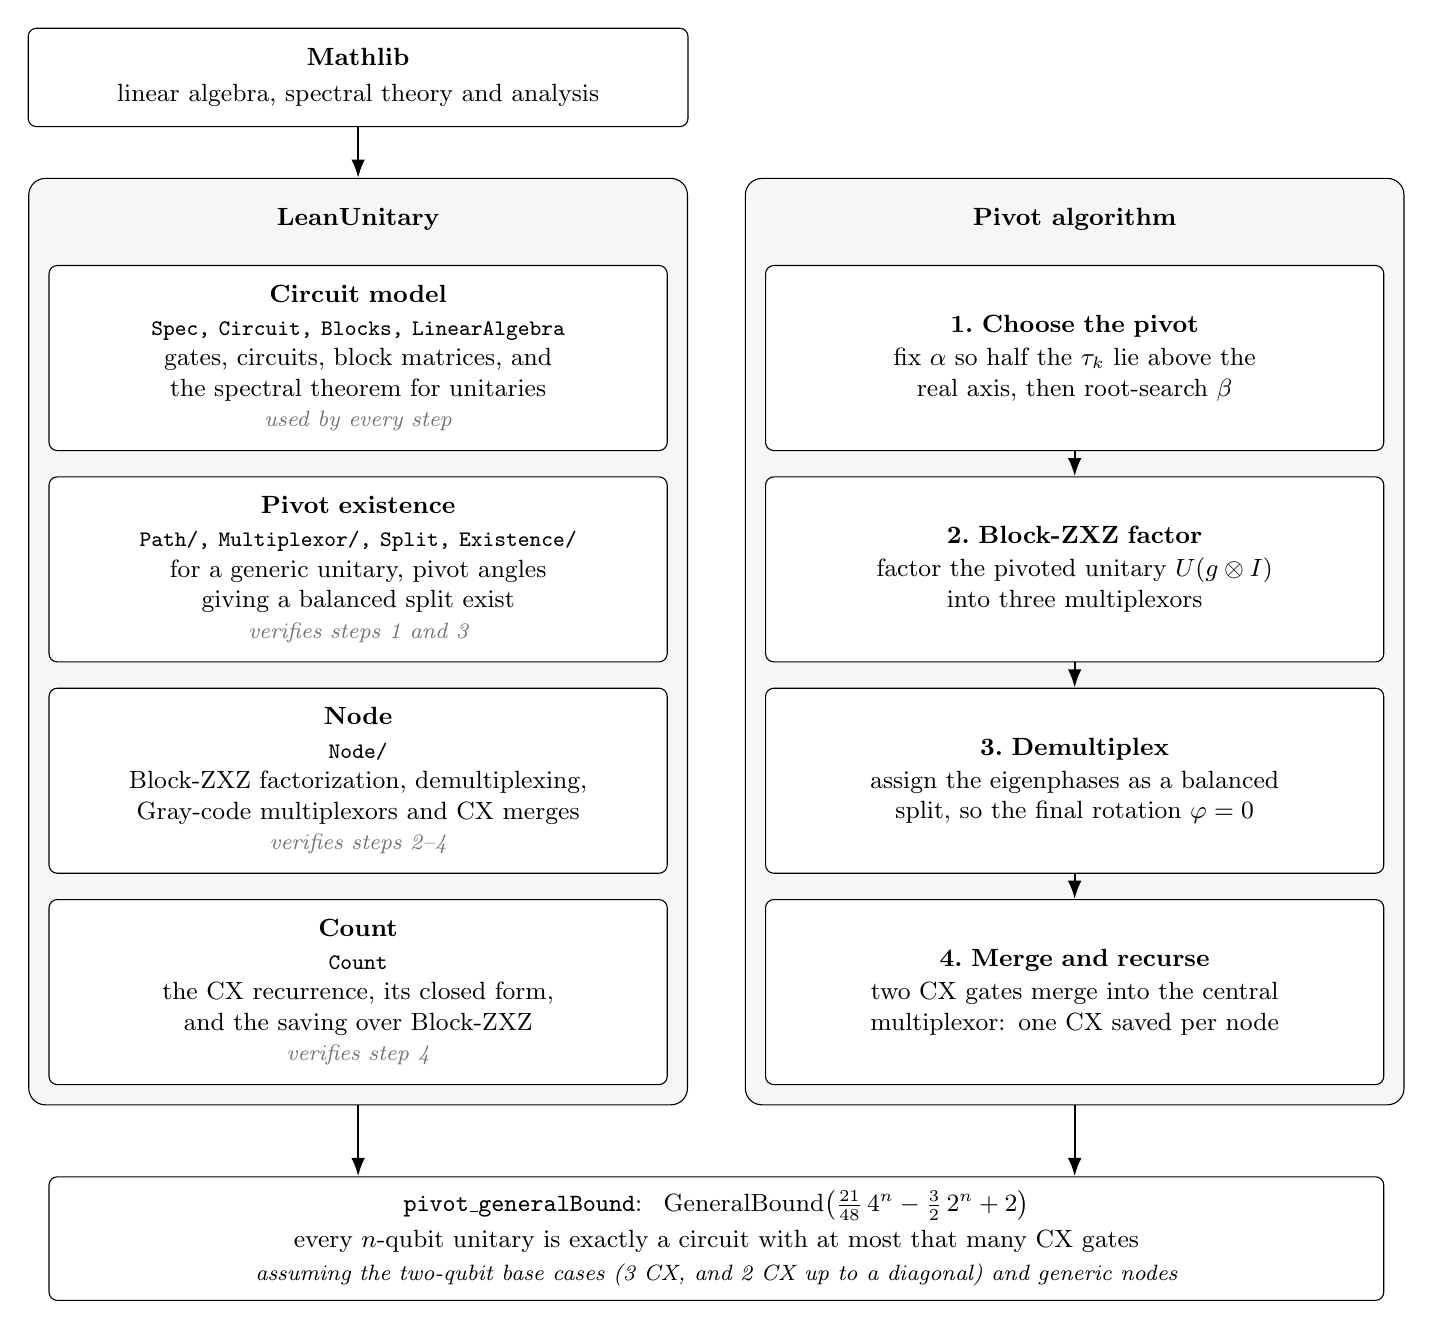
\begin{tikzpicture}[
    >=Latex,
    font=\small,
    box/.style={
        draw,
        rounded corners=3pt,
        align=center,
        inner sep=5pt,
        fill=white
    },
    col/.style={box, text width=7.5cm},
    wide/.style={box, text width=16.6cm, minimum height=1.25cm},
    head/.style={font=\small\bfseries, text width=7.5cm, align=center},
    arrow/.style={->, thick}
]

\def\xl{-4.55}
\def\xr{4.55}
\def\dx{9.1}
\coordinate (xl) at (\xl, 0);
\coordinate (xr) at (\xr, 0);

% ============================================================
% THEOREMS (left) VERIFY THE ALGORITHM (right)
% ============================================================

\node[head] (hl) at (\xl, -3.3) {LeanUnitary};
\node[head] (hr) at (\xr, -3.3) {Pivot algorithm};

% #1 row index, #2 node above, #3 left block, #4 right step; all rows share one height
\newcommand{\row}[4]{%
    \node[col, minimum height=2.35cm, anchor=north] (l#1) at ($(xl |- #2.south) + (0, -0.32)$) {#3};
    \node[col, minimum height=2.35cm, anchor=north] (a#1) at ($(xr |- #2.south) + (0, -0.32)$) {#4};
}

% modules, and the algorithm steps they verify
\newcommand{\mods}[1]{{\footnotesize\ttfamily #1}}
\newcommand{\vtag}[1]{{\footnotesize\color{black!55}\itshape #1}}

\row{1}{hl}
    {\step{Circuit model}{\mods{Spec, Circuit, Blocks, LinearAlgebra}\\gates, circuits, block matrices, and\\the spectral theorem for unitaries\\\vtag{used by every step}}}
    {\step{1.\ Choose the pivot}{fix $\alpha$ so half the $\tau_k$ lie above the\\real axis, then root-search $\beta$}}
\row{2}{l1}
    {\step{Pivot existence}{\mods{Path/, Multiplexor/, Split, Existence/}\\for a generic unitary, pivot angles\\giving a balanced split exist\\\vtag{verifies steps 1 and 3}}}
    {\step{2.\ Block-ZXZ factor}{factor the pivoted unitary $U(g\otimes I)$\\into three multiplexors}}
\row{3}{l2}
    {\step{Node}{\mods{Node/}\\Block-ZXZ factorization, demultiplexing,\\Gray-code multiplexors and CX merges\\\vtag{verifies steps 2--4}}}
    {\step{3.\ Demultiplex}{assign the eigenphases as a balanced\\split, so the final rotation $\varphi=0$}}
\row{4}{l3}
    {\step{Count}{\mods{Count}\\the CX recurrence, its closed form,\\and the saving over Block-ZXZ\\\vtag{verifies step 4}}}
    {\step{4.\ Merge and recurse}{two CX gates merge into the central\\multiplexor: one CX saved per node}}

\foreach \i [evaluate=\i as \j using int(\i+1)] in {1,...,3} {
    \draw[arrow] (a\i.south) -- (a\j.north);
}

\begin{scope}[on background layer]
\node[draw, rounded corners=6pt, fill=gray!7, inner sep=0.25cm,
    fit=(hl) (l1) (l4)] (lean) {};
\node[draw, rounded corners=6pt, fill=gray!7, inner sep=0.25cm,
    fit=(hr) (a1) (a4)] (alg) {};
\end{scope}

% Mathlib, the only dependency, directly above the LeanUnitary box and as wide
\node[draw, rounded corners=3pt, fill=white, inner sep=0pt,
    fit={($(lean.north west) + (0, 0.65)$) ($(lean.north east) + (0, 1.9)$)}] (mathlib) {};
\node[align=center] at (mathlib.center) {\textbf{Mathlib}\\[2pt]linear algebra, spectral theory and analysis};
\draw[arrow] (mathlib.south) -- (lean.north);

% ============================================================
% CLAIM
% ============================================================

\node[wide, below=0.9cm of $(lean.south)!0.5!(alg.south)$] (claim) {
    \mbox{\textbf{\texttt{pivot\_generalBound}}: \
    $\mathrm{GeneralBound}\big(\tfrac{21}{48}\,4^n-\tfrac32\,2^n+2\big)$}\\[2pt]
    every $n$-qubit unitary is exactly a circuit with at most that many CX gates\\[1pt]
    {\footnotesize\itshape assuming the two-qubit base cases (3 CX, and 2 CX up to a diagonal) and generic nodes}
};

\draw[arrow] (lean.south) -- (lean.south |- claim.north);
\draw[arrow] (alg.south) -- (alg.south |- claim.north);

\end{tikzpicture}

\caption{
Lean formalization of the pivot decomposition. The modules of LeanUnitary (left) are
tagged with the steps of the pivot algorithm (right) they verify.
}

\label{fig:lean-unitary}

\end{figure}

\end{document}
